\chapter{Čiernobiele obrázky}
\label{sec:CB obrazky}

Dvojrozmerné pole núl a jednotiek sa dá chápať ako čiernobiely obrázok, kde 1 je biela
a 0 čierna. Aby sa dali lepšie pozerať, môžeš si stiahnuť súbor 
\link{\rootpath/obrazok.h}{obrazok.h}, v ktorom som ti
pripravil\footnote{V skutočnosti som len použil program \vb{lodePNG}, ktorý je
voľne prístupný a vie zapisovať obrázky vo formáte PNG.} 
príkaz na zapísanie dvojrozmerného poľa do obrázku. Ukážem ti, ako sa s ním
pracuje. Povedzme, že chceme urobiť obrázok rozmerov $300\times200$, ktorý bude mať
v strede čierny štvorec rozmerov $80\times80$ takto:\\


\centerline{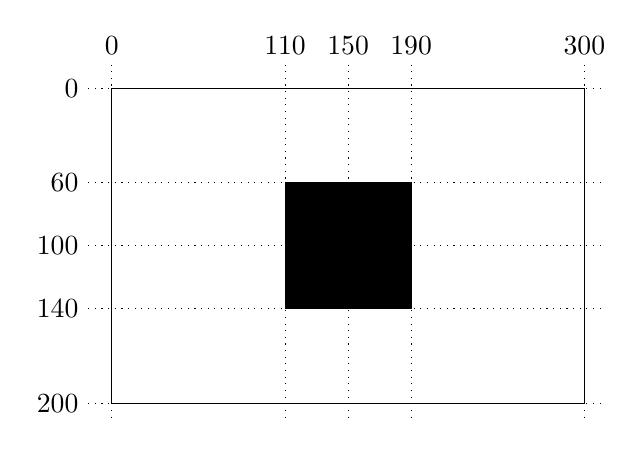
\begin{tikzpicture}[xscale=0.02,yscale=-0.02]
  \def\d{15}
  \def\hl#1{
    \draw[dotted] (-\d,#1) node[anchor=east]{#1} -- (310,#1);
  }
  \def\vl#1{
    \draw[dotted] (#1,-\d)node[anchor=south]{#1} -- (#1,210);
  }
  \draw (0,0) rectangle (300,200);
  \filldraw (110,60) rectangle (190,140);
  \hl0
  \hl{100}
  \hl{200}
  \hl{140}
  \hl{60}
  \vl0
  \vl{300}
  \vl{150}
  \vl{110}
  \vl{190}
\end{tikzpicture}}

Začni tým, že si súbor \vb{obrazok.h} ulož do toho istého adresára, kde máš program
a napíš:\\

\vbox{
\begin{lstlisting}[] 
#include <iostream>
#include "obrazok.h"

int main() {
  int a[200][300], i, j;
  for (i = 0; i < 200; i++)
    for (j = 0; j < 300; j++)
      if (i >= 60 && i <= 140 && j >= 110 && j <= 190)
        a[i][j] = 0;
      else
        a[i][j] = 1;
  zapis_cb_png(200, 300, a, "vystup.png");
}
\end{lstlisting}
}

V druhom riadku hovoríš, že sa má použiť súbor \vb{obrazok.h}. V poslednom riadku
používaš príkaz \hbox{\vb{zapis\_cb\_png},} ktorý je naprogramovaný v tom súbore a má tri parametre, ktoré
sa píšu v zátvorkách:
počet riadkov, počet stĺpcov, dvojrozmerné pole núl a jednotiek a meno výstupného
súboru. Zvyšok by mal byť jasný: premennou \prg!i! prechádzame v cykle cez všetky riadky,
pre každý riadok premennou \prg!j! prechádzame cez všetky stĺpce. 
Pre každé políčko poľa zistíme, aká farba tam má byť, a zapíšeme.
Keď program skompiluješ a spustíš, vyrobí ti súbor \vb{vystup.png}, ktorý
sa dá pozrieť v prehliadači obrázkov.

\begin{uloha}
  Napíš program, ktorý načíta čísla $n$ a $d$ a vyrobí štvorcový obrázok rozmerov 
  $n\times n$ s čiernym rámikom hrúbky $d$.
\end{uloha}

\begin{uloha}
  Napíš program, ktorý prečíta číslo $d$ a spraví obrázok rozmerov $d\times d$
  s čiernym trojuholníkom takto:\\

  
  \centerline{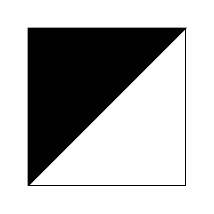
\begin{tikzpicture}[scale=2]
    \draw (0,0) rectangle (1,1);
    \filldraw (0,0) -- (1,1) -- (0,1) -- (0,0);
  \end{tikzpicture}
  }
\end{uloha}


\begin{uloha}
  Napíš program, ktorý prečíta čísla $n$, $d$ a vyrobí obrázok so štvorcovou
  mriežkou $n\times n$ a rozostupmi $d$. Napr. pre $n=301$ a $d=15$ bude obrázok:\\

  
\centerline{
\includegraphics[width=4cm]{data/grid.png}}

\end{uloha}


\begin{uloha}
  Napíš program, ktorý prečíta číslo $d$ a vyrobí obrázok šachovnice ($8\times 8$
  políčok, v ľavom dolnom rohu je čierne políčko) rozmerov $8d\times 8d$, ktorej
  jedno políčko má rozmery $d\times d$.
\end{uloha}


\section*{Malá odbočka: Pytagorova veta, Euklidova vzdialenosť a kruhy}
\label{mat.pytagoras}

\indexItem{Mat}{Pytagorova veta}
Poznáš Pytagorovu vetu? Nie je nová, starí Gréci ju poznali viac ako 300 rokov pr. Kr. 
Asi vieš, že obsah štvorca so stranou $x$ sa dá vypočítať ako $x\cdot x=x^2$.
Pytagorova veta hovorí, že v pravouhlom trojuholníku sa obsah štvorca nad preponou
rovná súčtu obsahov štvorcov nad odvesnami. Alebo kratšie, $c^2=a^2+b^2$:\\


\centerline{
  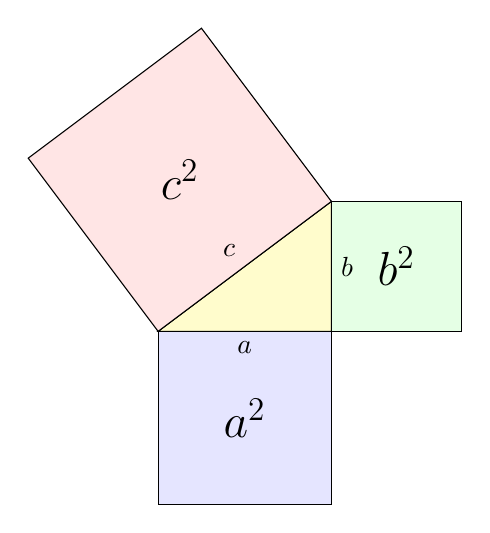
\begin{tikzpicture}[scale=0.55]
    \filldraw[fill=yellow!20!white] (0,0) -- (4,0) -- (4,3) -- cycle;
    \filldraw[fill=blue!10!white] (0,0) -- (4,0) -- (4,-4) -- (0,-4) -- cycle;
    \filldraw[fill=green!10!white] (4,0) -- (7,0) -- (7,3) -- (4,3) -- cycle;
    \filldraw[fill=red!10!white] (0,0) -- (-3,4) -- (1,7) -- (4,3) -- cycle;
    \draw (2,0) node[anchor = north] {$a$};
    \draw (4,1.5) node [anchor=west] {$b$};
    \draw (2,1.5) node [anchor=south east] {$c$};
    \draw (0.5,3.5) node [anchor=center] {\textcolor{black}{\LARGE $c^2$}};
    \draw (2,-2) node [anchor=center] {\textcolor{black}{\LARGE $a^2$}};
    \draw (5.5,1.5) node [anchor=center] {\textcolor{black}{\LARGE $b^2$}};
  \end{tikzpicture}
}

 Prečo to platí ľahko vidno z nasledujúceho obrázka. 
Vľavo sú štyri rovnaké trojuholníky naukladané do štvorca. 
Pri každom bode v strede strany sú dva rôzne uhly z trojuholníkov,
ktoré dokopy dajú $90^\circ$ (súčet uhlov v trojuholníku je $180^\circ$).
Preto biela vec vovnútri je štvorec.
Vo veľkom štvorci sa iba premiestnili
farebné trojuholníky a vznikol obrázok vpravo, takže plocha bielej časti v oboch 
obrázkoch musí byť rovnaká:


\centerline{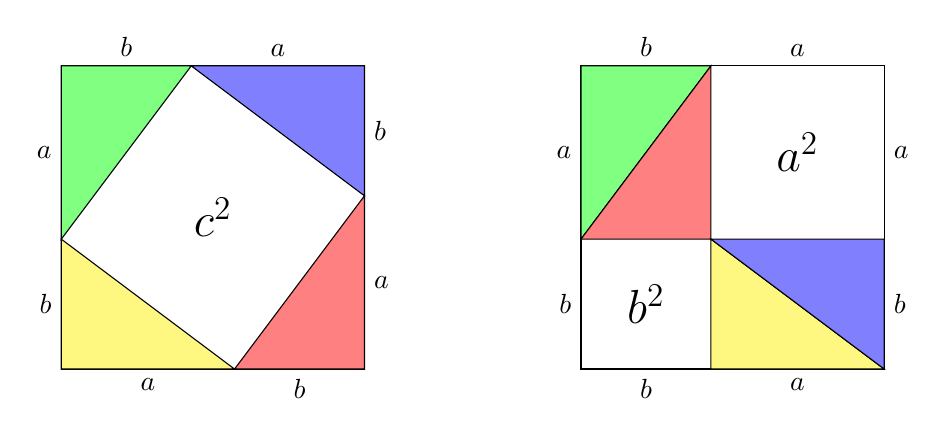
\begin{tikzpicture}[scale=0.55]
  \draw (0,0) rectangle (7,7);
  \filldraw[fill=yellow!50!white] (0,3) -- (0,0) -- (4,0) -- cycle;
  \filldraw[fill=red!50!white] (4,0) -- (7,0) -- (7,4) -- cycle;
  \filldraw[fill=blue!50!white] (7,4) -- (7,7) -- (3,7) -- cycle;
  \filldraw[fill=green!50!white] (3,7) -- (0,7) -- (0,3) -- cycle;
  
  \draw (2,0) node[anchor=north] {$a$};
  \draw (5.5,0) node[anchor=north] {$b$};
  \draw (5,7) node[anchor=south] {$a$};
  \draw (1.5,7) node[anchor=south] {$b$};
  \draw (0,1.5) node[anchor=east]{$b$};
  \draw (7,2) node[anchor=west]{$a$};
  \draw (0,5) node[anchor=east]{$a$};
  \draw (7,5.5) node[anchor=west]{$b$};

  \draw (3.5,3.5) node[anchor=center]{{\LARGE $c^2$}};

  \begin{scope}[shift={(12,0)}]
    \draw (0,0) rectangle (7,7);
    \filldraw[fill=green!50!white] (3,7) -- (0,7) -- (0,3) -- cycle;
    \filldraw[fill=red!50!white] (0,3) -- (3,3) -- (3,7) -- cycle;
    \filldraw[fill=yellow!50!white] (3,3) -- (3,0) -- (7,0) -- cycle;
    \filldraw[fill=blue!50!white] (7,0) -- (7,3) -- (3,3) -- cycle;
  
    \draw (0,1.5) node[anchor=east]{$b$};
    \draw (0,5) node[anchor=east]{$a$};
    \draw (5,7) node[anchor=south] {$a$};
  \draw (1.5,7) node[anchor=south] {$b$};
    \draw (7,1.5) node[anchor=west]{$b$};
    \draw (7,5) node[anchor=west]{$a$};
    \draw (5,0) node[anchor=north] {$a$};
  \draw (1.5,0) node[anchor=north] {$b$};
    \draw (1.5,1.5) node[anchor=center]{{\LARGE $b^2$}};
    \draw (5,5) node[anchor=center]{{\LARGE $a^2$}};

  \end{scope}
  
\end{tikzpicture}\\
}

Pytagorova veta zároveň hovorí\footnote{%
  keďže $c^2=a^2+b^2$, tak $c=\sqrt{a^2+b^2}$. \indexItem{Mat}{odmocnina}Znak $\sqrt{x}$ sa číta \cmd{odmocnina
  z $x$} a znamená \cmd{číslo, ktoré keď umocním na druhú (t.j. vynásobím samé so sebou)
  dostanem $x$}, t.j $(\sqrt{x})^2=\sqrt{x}\cdot\sqrt{x}=x$. Napríklad $\sqrt{36}=6$.
  }, že ak mám v rovine dva body, bod $A$ so súradnicami
$[x_1,y_1]$ a bod $B$ so súradnicami $[x_2,y_2]$, tak ich vzdialenosť je \indexItem{Mat}{vzdialenosť bodov}
$\sqrt{(x_2-x_1)^2+(y_2-y_1)^2}$:\\


\centerline{\begin{tikzpicture}[scale=0.8]
  \filldraw (0,0) circle (1pt) node[anchor=east] {$A=[x_1,y_1]$};
  \filldraw (4,3) circle (1pt) node[anchor=south west] {$B=[x_2,y_2]$};
  \draw(0,0)--(4,3);
  \draw[dotted] (0,0) -- (4,0) -- (4,3);
    
    \draw[blue] decorate[
       decoration={brace, amplitude=2ex}]{
       (4,0) -- (0,0) node [align=center,midway,anchor=south,shift={(0,-0.8)}] {$x_2-x_1$}
        };
    \draw[red] decorate[
       decoration={brace, amplitude=2ex}]{
       (4,3) -- (4,0) node [align=center,midway,anchor=west,xshift=2ex] {$y_2-y_1$}
        };
\end{tikzpicture}}


No a napokon kruh so stredom v bode $S=[x,y]$ a polomerom $r$ je tvorený bodmi
$X=[x',y']$, pre ktoré vzdialenosť od $S$ je nanajvýš $r$, takže platí
$(x-x')^2+(y-y')^2\le r^2$. S týmto už ľahko vyriešiš túto úlohu:

\begin{uloha}
  \label{uloha:kruh}
Na vstupe sú čísla $a$ a $r$. Napíš program, ktorý vyrobí obrázok 
rozmerov $a\times a$, ktorý bude mať v strede kruh s polomerom $r$.
Napr. pre $a=300$, $r=100$ bude obrázok vyzerať takto:\\

  {
  \setlength{\fboxsep}{0pt}
\centerline{\fbox{
\includegraphics[width=3cm]{data/kruh.png}}}
  }

\end{uloha}

\section*{Projekt: Celulárny automat}
\label{projekt.automat}

Máme kolóniu baktérií, ktoré žijú na čiare. 
Na začiatku je živá iba jedna baktéria:

\centerline{\vb{..........*..........}}


V každej ďalšej generácii sa kolónia vyvíja podľa nasledovných pravidiel: 
\begin{enumerate}\itemsep=-1mm
    \item ak je na políčku baktéria, ktorá má dvoch susedov, tak skape, lebo nemá dosť miesta
    \item ak je prázdne políčko, ktoré nesusedí s baktériou, ostane prázdne
    \item vo všetkých ostatných prípadoch na políčku bude baktéria
\end{enumerate}

Prvé štyri generácie budú vyzerať takto:

\centerline{\vb{0: ..........*..........}}
\centerline{\vb{1: .........***.........}}
\centerline{\vb{2: ........**.**........}}
\centerline{\vb{3: .......*******.......}}
\centerline{\vb{4: ......**.....**......}}

\begin{uloha}
Napíš program, ktorý načíta $n$ a $t$, pričom $t<n$ a vypíše jeden riadok dĺžky $2n+1$
z bodiek a hviezdičiek, ktorý
bude znázorňovať, ako bude kolónia vyzerať po $t$ generáciách.
\end{uloha}

\begin{uloha}
  Napíš program, ktorý prečíta $t$ a vykreslí obrázok rozmerov $(2t+1)\times t$, v ktorom
  $i$-ty riadok bude zodpovedať $i$-tej generácii: ak je na políčku baktéria, bude tam 
  čierny pixel,
  inak biely. Prvý riadok bude celý biely, iba v strede (na pozícii $[0][t]$) bude
  čierny pixel.
\end{uloha}

 Môžeme ďalej skúmať, ako by vyzeral náš obrázok, keby kolónia mala iné pravidlá.
Políčko má  osem možností, ako môže vyzerať jeho okolie:


\centerline{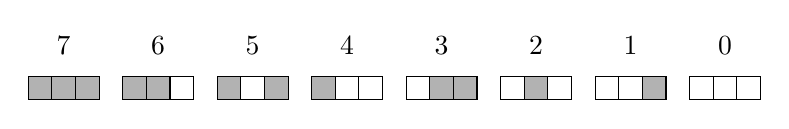
\begin{tikzpicture}[scale=0.3]
  \def\n#1#2{
    \filldraw[fill=\if#10white\else black!30!white\fi] (#2,0) rectangle (#2+1,1);
  }
  \def\N#1#2#3#4{
    \draw(1.5,1.5) node[anchor=south] {$#4$};
    \n#10\n#21\n#32
  }
  
  \foreach \v [count = \i] in {0000,0011,0102,0113,1004,1015,1106,1117} {
    \begin{scope}[shift={(-4*\i,0)}]
      \expandafter\N\v
    \end{scope}
  }
\end{tikzpicture}}


Ak si všimneš, očísloval som ich tak, že ak plné políčko je jednotka a prázdne políčko je 
nula, tak políčka vlastne tvoria číslo okolia zapísané v dvojkovej sústave, napr. okolie
s číslom 5 je
\vb{101}. Inak povedané, ak mám tri čísla (nuly a jednotky) 
$x,y,z$, tak číslo okolia je $4x+2y+z$.


Pravidlo pre rast kolónie musí pre každé okolie povedať, či v ňom v ďalšej generácii
bude baktéria alebo nie. Naše pravidlo vyzerá takto:


\centerline{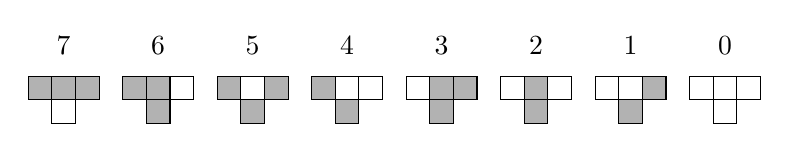
\begin{tikzpicture}[scale=0.3]
  \def\n#1#2{
    \filldraw[fill=\if#10white\else black!30!white\fi] (#2,0) rectangle (#2+1,1);
  }
  \def\N#1#2#3#4#5{
    \draw(1.5,1.5) node[anchor=south] {$#4$};
    \n#10\n#21\n#32
    \begin{scope}[shift={(1,-1)}]\n#50\end{scope}
  }
  
  \foreach \v [count = \i] in {00000,00111,01021,01131,10041,10151,11061,11170} {
    \begin{scope}[shift={(-4*\i,0)}]
      \expandafter\N\v
    \end{scope}
  }
\end{tikzpicture}}


Každé pravidlo viem opísať pomocou 8 núl alebo jednotiek, ktoré hovoria výsledok pre 
jednotlivé okolia. Naše pravidlo je \vb{01111110}. Keď si predstavíme, 
že to je zápis nejakého čísla v dvojkovej sústave, každé z 256 možných
pravidiel kolónie môžeme označiť číslom z rozsahu $0$ až $255$.
Naše pravidlo je


\centerline{\begin{tikzpicture}
  \foreach \v/\p [count=\i] in { 0/128, 1/64, 1/32, 1/16, 1/8, 1/4, 1/2, 0/1} {
    \draw[dotted, shorten <= 2ex, shorten >= 2ex] 
    (\i,0) node [color=green!70!black] {{\small \p}}
     -- (\i,-6ex) node {\v};
  }
\end{tikzpicture}}

\indexItem{Prg}{bitové operácie}
$64+32+16+8+4+2=126$. Našim cieľom teraz bude preskúmať rôzne pravidlá.
Ako ľahko pracovať s číslom pravidla? Na to pomôžu tzv. {\em bitové operácie}. Sú to
operácie nad celými číslami (podobne ako \vb{+,-,*,/,\%}), ale pracujú s jednotlivými
bitmi čísla v dvojkovej sústave.\\

\def\prikl#1#2#3{\raisebox{-1.5cm}{%
  \begin{tikzpicture}[scale=0.45]
    \def\p(##1,##2)##3{\draw[draw=none] (##1,##2) 
    rectangle node[align=center]{\vb{##3}} (##1+1,##2+1);
    }
    \foreach \x[count=\i] in {8, 4, 2, 1}{
      \draw[draw=none] (\i,1) rectangle node[color=green!60!black, align=center]
      {{\scriptsize\roboto \x}} (\i+1,2);
    }
    \p(0,0){#1:}
    \foreach \x [count=\i] in \opA {\p(\i,0){\x}}
    \p(0,-1){#2:}
    \foreach \x [count=\i] in \opB {\p(\i,-1){\x}}
    \draw (0,-1.2) -- (5,-1.2);
    \p(0,-2.2){#3:}
    \foreach \x [count=\i] in \res {\p(\i,-2.2){\x}}
  \end{tikzpicture}}
}



\centerline{\begin{tabular}{|c|c|p{7cm}|l|p{2.5cm}|}\hline
\vb{\&} & AND & 
  výsledok je číslo, ktoré má bit nastavený na 1, ak obe čísla majú
  príslušný bit 1
  & \vb{10 \& 9 == 8} &
\global\def\opA{1,0,1,0}
\global\def\opB{1,0,0,1}
\global\def\res{1,0,0,0}
  \prikl{10}{9}{8} \\\hline
\vb{|} & OR & 
  výsledok je číslo, ktoré má bit nastavený na 1, ak aspoň jedno číslo má
  príslušný bit 1
  & \vb{10 | 9 == 11} &
\global\def\opA{1,0,1,0}
\global\def\opB{1,0,0,1}
\global\def\res{1,0,1,1}
  \prikl{10}{9}{11} \\\hline
  \vb{\^{}} & XOR & 
  výsledok je číslo, ktoré má bit nastavený na 1, ak práve jedno číslo má
  príslušný bit 1
  & \vb{10 \^{} 9 == 3} &
\global\def\opA{1,0,1,0}
\global\def\opB{1,0,0,1}
\global\def\res{0,0,1,1}
  \prikl{10}{9}{3} \\\hline
\end{tabular}}


Ešte sa hodia dve bitové operácie. Operácia \prg!<<! posúva binárny zápis čísla doľava.
\prg!x << a! pripíše \vb{a} núl na koniec dvojkového\footnote{\phantomsection\label{foot:hexa2}%
Tu sa prejaví výhoda $16$-kovej sústavy. Pretože $16=2^4$, jedna cifra v $16$-kovej sústave priamo
zodpovedá štyrom binárnym cifrám. Takže napr. \vb{0xff<<8} je \vb{255<<8}, t.j. 
$255\cdot2^8=255\cdot256=65280$, čo je \vb{0xff00}. 
}zápisu \vb{x}. To je to isté,
ako keby som ho \vb{a}-krát za sebou vynásobil dvomi. Napr $5$ je v dvojkovej sústave
\vb{101}. \prg!5 << 3! preto bude číslo s dvojkovým zápisom \vb{101000}, čo je
$5\cdot8=40$. Opačná operácia \prg!>>!posúva číslo doprava, t.j. zoberie celú časť po delení dvomi.
Napr. $45$ je v dvojkovej sústave \vb{101101}. Keď ho trikrát vydelím dvomi a vždy zoberiem celú časť, dostanem
\vb{10110} (čo je $22$), \vb{1011} (čo je $11$) a \vb{101} (čo je $5$). Preto \prg!45 >> 3! je $5$. 


S týmito operáciami viem jednoducho vyhodnocovať pravidlá. Predpokladajme, že mám
pravidlo \prg!r! a niekde
v poli mám hodnoty políčok \prg!a[i-1]!, \prg!a[i]!, \prg!a[i+1]!. 
Číslo okolia (od 0 do 7) dostanem tak, že
vyrátam \hbox{\prg!z = 4 * a[i-1] + 2 * a[i] + a[i+1]!}. 
Bit na pozícii \vb{z} v pravidle mi hovorí, či bude políčko v ďalšej generácii 
obsadené. Preto stačí vyrátať \prg!r & (1 << z)!, t.j. jednotku posunúť o \vb{z}
pozícií doprava a urobiť operáciu AND s pravidlom. Ak je výsledok 0, políčko má byť
prázdne. Ak je výsledok nenulový (t.j rovný \prg!1 << z!), na políčku bude baktéria.

\begin{uloha}
  Napíš program, ktorý načíta číslo pravidla $r$ a počet iterácií $t$ a vyrobí obrázok
  (rozmerov $2t+1\times t$),
  ako vyzerá vývoj kolónie s pravidlom $r$ počas $t$ generácií.
\end{uloha}


Môžeš skúmať rôzne pravidlá: niektoré kolónie rýchlo vymrú, niektoré vyrobia jednoduché útvary 
(napr. čiaru), iné robia tzv. deterministický chaos, a ešte iné rôzne pravidelné
obrazce. Niekoľko pravidiel je tu\footnote{Všimni si, že párne pravidlo vytvorí biele pozadie a nepárne pravidlo pásikavé. Je to náhoda? Vieš povedať,
prečo to tak je?}:


\vbox{
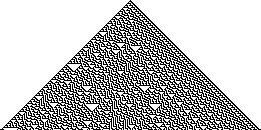
\includegraphics[width=7cm]{data/r86.png}
\hfill
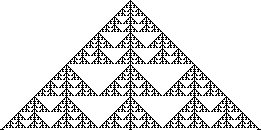
\includegraphics[width=7cm]{data/r150.png}\\
\hbox to 7cm{\hss pravidlo 86\hss}
\hfill
\hbox to 7cm{\hss pravidlo 150\hss}
}

\vskip 1ex

\vbox{
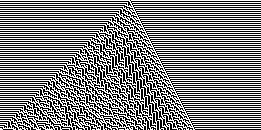
\includegraphics[width=7cm]{data/r89.png}
\hfill
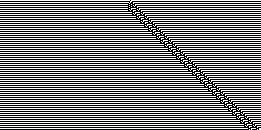
\includegraphics[width=7cm]{data/r107.png}\\
\hbox to 7cm{\hss pravidlo 89\hss}
\hfill
\hbox to 7cm{\hss pravidlo 107\hss}
}


Rovnako dobre sa dá skúšať, čo sa stane, ak kolónia nezačína z jednej baktérie, ale z 
niekoľkých, ako sa správajú dve rastúce kolónie, ktoré do seba narazia, čo ak 
je pravidlo z väčšieho okolia a pod.

